\documentclass[11pt]{article}
\usepackage[margin=1.0in]{geometry}
\usepackage{lmodern}
\usepackage{microtype}
\usepackage{amsmath,amssymb}
\usepackage{graphicx}
\usepackage{booktabs}
\usepackage{longtable}
\usepackage{array}
\usepackage[table]{xcolor}
\usepackage{caption}
\usepackage{enumitem}
\usepackage{tikz}
\usetikzlibrary{arrows.meta,positioning,shapes.geometric}
\usepackage[colorlinks=true,linkcolor=teal,urlcolor=teal,citecolor=teal]{hyperref}
\usepackage{titlesec}
\usepackage{fancyhdr}

\captionsetup{font=small,labelfont=bf,skip=5pt}
\titlespacing{\section}{0pt}{13pt}{5pt}
\titlespacing{\subsection}{0pt}{9pt}{3pt}
\setlength{\parskip}{3pt}
\setlength{\parindent}{0pt}

\definecolor{v1c}{HTML}{C0561F}
\definecolor{v15c}{HTML}{8A6D3B}
\definecolor{v2c}{HTML}{20699F}
\definecolor{boxbg}{HTML}{F4F7FA}
\definecolor{warnbg}{HTML}{FDF3E3}

\newcommand{\co}{$^\circ$C}
\newcommand{\mdot}{\dot m}
\newcommand{\file}[1]{\texttt{\small #1}}

% callout boxes
\newcommand{\keybox}[2]{%
  \begin{center}\colorbox{boxbg}{\begin{minipage}{0.94\linewidth}\vspace{3pt}
  \textbf{#1}\\[2pt]#2\vspace{3pt}\end{minipage}}\end{center}}
\newcommand{\warnbox}[2]{%
  \begin{center}\colorbox{warnbg}{\begin{minipage}{0.94\linewidth}\vspace{3pt}
  \textbf{#1}\\[2pt]#2\vspace{3pt}\end{minipage}}\end{center}}

\pagestyle{fancy}\fancyhf{}
\fancyhead[L]{\small CFD v2 --- Air-Side Heater Unit Cell}
\fancyhead[R]{\small Phase 1, Stream A}
\fancyfoot[C]{\small\thepage}
\renewcommand{\headrulewidth}{0.4pt}
\setcounter{tocdepth}{1}
\setlength{\emergencystretch}{3em}

\title{\vspace{-1.4em}\textbf{CFD of the Air-Cooled Heater of a\\Heat-Pipe Microreactor}\\[4pt]
\large Validating the Air-Side Heat-Transfer Law Behind the\\Saudi Desert Derating Curve}
\author{\normalsize Omar \quad$\cdot$\quad Supervisor: Dr.\ Salman Alshehri\\[-1pt]
\small KACST Nuclear Technologies Institute \,/\, King Abdulaziz University\\[-1pt]
\small Co-operative Training Program, 2026}
\date{\small Combined Microreactor Project --- Phase 1 (Physics / Derating), Stream A}

\begin{document}
\maketitle
\thispagestyle{fancy}
\vspace{-1.6em}

\noindent\rule{\linewidth}{0.4pt}
\begin{abstract}\noindent\small
A Westinghouse eVinci-class heat-pipe microreactor (15\,MW$_\mathrm{th}$ / 5\,MW$_\mathrm{e}$) rejects no
water: it converts reactor heat with a recuperated \emph{open-air} Brayton cycle whose compressor breathes
ambient air directly. That is precisely what makes it suitable for arid Saudi siting, and precisely what makes
it sensitive to desert heat. Phase~1 of this project quantifies that sensitivity as a \emph{derating curve} ---
net electric output versus ambient temperature over 25--55\,\co --- which Phase~2 then consumes as a
physics-grounded, per-site input to a nuclear siting study.

This report documents the CFD campaign within Phase~1. The cycle model had one unverified assumption left: how
the air-cooled finned-tube heater's conductance $UA$ scales with air mass flow, assumed as $UA\propto\mdot^{0.6}$.
A steady compressible OpenFOAM solve (\file{rhoSimpleFoam} + $k$--$\omega$ SST, 3.29\,M cells) of a staggered
finned-tube unit cell at the cycle design Reynolds number $Re=8368$ measured the air-side heat transfer and
validated it against the Briggs--Young correlation: $Nu_\mathrm{CFD}=45.9$ vs $Nu_\mathrm{BY}=54.1$, a
$-15.2\%$ deviation inside the project's $\pm20\%$ engineering gate. The validated law, converted to a heater
$UA(\mdot)$ and modulated by fin efficiency, gives an effective exponent $n=0.454$ --- materially
\emph{shallower} than the assumed $0.6$, contrary to first expectation. Injecting it into the cycle model moves
the 55\,\co{} penalty from $-8.75\%$ to $-8.67\%$: a $0.08$-percentage-point change.

The null result is the finding. Because ambient temperature swings the Brayton air mass flow by only
$\sim$4--5\% across 25--55\,\co, the air-side exponent is a second-order term: sweeping it over the entire
physically plausible range $n\in[0,1.2]$ moves the penalty by just $0.66$ points. The desert derating is
therefore set by compressor-inlet thermodynamics, not by heat-exchanger detail, and is \emph{robust} to the
heater law assumed. Friction did not validate ($f_\mathrm{CFD}=1.688$ vs $0.287$, $+489\%$, a
measurement-domain mismatch) and is excluded from the power balance. The durable asset is a validated OpenFOAM
air-side setup, now available for the intake/exhaust recirculation study that no correlation can address.
\end{abstract}
\noindent\rule{\linewidth}{0.4pt}

\vspace{4pt}
{\small\tableofcontents}
\clearpage


% =====================================================================
\part*{Part I --- Project Context}
\addcontentsline{toc}{section}{\textbf{Part I --- Project Context}}
% =====================================================================

\section{What the overall project is trying to answer}

The project merges two research proposals into one study with a single connecting thread.

\begin{description}[leftmargin=1.6em,itemsep=3pt]
\item[Phase 1 --- \emph{the desert thermal penalty}.] How much output does an air-cooled heat-pipe
microreactor lose in Saudi ambient conditions (25--55\,\co)? The deliverable is a physics-based
\textbf{derating curve}: net electric power and efficiency as a function of ambient temperature.
\item[Phase 2 --- \emph{siting feasibility}.] Where in Saudi Arabia should such a reactor go, for which
application (mining, desalination, industrial, remote electrification), and at what power class? The
deliverable is a decision-support framework (AHP scoring $\rightarrow$ Random Forest $\rightarrow$ SHAP
explainability) over 30--80 named Saudi sites.
\end{description}

The connection is what makes the study novel. Published siting studies treat ``climate'' as a heuristic
scoring criterion --- typically a fixed weight of around 10\% in an AHP matrix, assigned by expert judgement.
Phase~1 replaces that heuristic with a computed, physics-grounded, per-site derating: each candidate site's
NASA POWER temperature climatology is pushed through the Phase-1 curve to yield that site's actual expected
capacity factor. The siting rankings then rest on thermodynamics rather than on an opinion about how much
heat matters. No published work provides this linkage.

\subsection{Why this reactor class is the interesting case}

The reference design is the \textbf{Westinghouse eVinci}, a heat-pipe microreactor whose facts are locked from
the IAEA ARIS 2024 datasheet (Table~\ref{tab:ref}). Two of its features interact in a way that is central to
the whole project:

\begin{enumerate}[leftmargin=1.6em,itemsep=2pt]
\item \textbf{It needs no cooling water.} Solid-core, sodium heat pipes, air-cooled. For a country siting
reactors in a desert, or next to a desalination plant that has better uses for water, this is the decisive
advantage.
\item \textbf{It uses an open-air Brayton cycle.} The power conversion system is effectively a ground-based
gas turbine: it draws its working fluid from the atmosphere, compresses it, heats it against the reactor's
heat pipes, expands it through a turbine, and exhausts it.
\end{enumerate}

Feature 2 is the price of feature 1. In an \emph{open-air} Brayton, the compressor-inlet temperature
\emph{is} the ambient temperature. Compressor work scales with inlet temperature ($w_c \propto T_1$), so on a
hot day the machine spends more of its turbine output just compressing air, and the air is less dense so it
swallows less mass flow. This is the well-known gas-turbine ``hot-day derating'' --- the same physics by which
cars and aircraft lose power in hot or thin air. The water-free design that suits arid siting is therefore
also the design most punished by desert heat, and the size of that penalty is exactly what Phase~1 must
determine.

Note where the sensitivity does \emph{not} live: the reactor core delivers its 15\,MW$_\mathrm{th}$ through
sodium heat pipes regardless of the weather. All ambient sensitivity is in the power conversion system. This
is why Phase~1 is a cycle-modelling and CFD problem rather than a neutronics problem.

\begin{table}[h]\centering\small
\caption{Reference design point (calibration v1.1). Reactor-scale facts from the IAEA ARIS 2024 datasheet;
the finned-tube heat-exchanger geometry is not public and was specified as a representative standard bank.}
\label{tab:ref}
\resizebox{\linewidth}{!}{%
\begin{tabular}{@{}llll@{}}
\toprule
Thermal / electric power & 15 / 5\,MW & Pressure ratio & 3.0\\
Power conversion & recuperated open-air Brayton & Compressor / turbine $\eta$ & 0.82 / 0.85\\
Turbine-inlet temperature (solved) & 742\,\co & Recuperator effectiveness & 0.88\\
Net efficiency @ 25\,\co & 33\% & Mechanical/parasitic $\eta_\mathrm{mech}$ & 0.93\\
Core life / fuel & 8 years, TRISO/graphite & Heat transport & sodium heat pipes\\
\bottomrule
\end{tabular}}
\end{table}

\subsection{How the derating curve was built, and where CFD enters}

The curve was developed in three generations, each removing exactly one assumption. This report concerns the
third.

\begin{center}
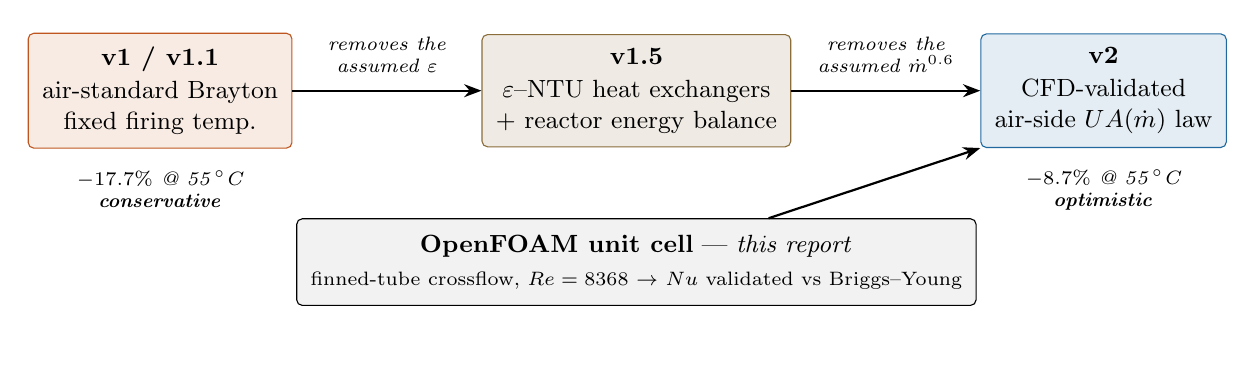
\begin{tikzpicture}[
  node distance=6mm,
  box/.style={draw,rounded corners=2pt,align=center,font=\small,inner sep=5pt,minimum height=11mm},
  lbl/.style={font=\scriptsize\itshape,align=center},
  ar/.style={-{Stealth[length=2.2mm]},thick}]
\node[box,fill=v1c!12,draw=v1c] (v1) {\textbf{v1 / v1.1}\\[1pt]air-standard Brayton\\fixed firing temp.};
\node[box,fill=v15c!14,draw=v15c,right=24mm of v1] (v15) {\textbf{v1.5}\\[1pt]$\varepsilon$--NTU heat exchangers\\+ reactor energy balance};
\node[box,fill=v2c!12,draw=v2c,right=24mm of v15] (v2) {\textbf{v2}\\[1pt]CFD-validated\\air-side $UA(\mdot)$ law};
\node[box,fill=black!5,below=9mm of v15] (cfd) {\textbf{OpenFOAM unit cell} --- \emph{this report}\\[1pt]
  \scriptsize finned-tube crossflow, $Re=8368$ $\rightarrow$ $Nu$ validated vs Briggs--Young};
\draw[ar] (v1) -- node[lbl,above,yshift=1mm]{removes the\\assumed $\varepsilon$} (v15);
\draw[ar] (v15) -- node[lbl,above,yshift=1mm]{removes the\\assumed $\mdot^{0.6}$} (v2);
\draw[ar] (cfd) -- (v2.south west);
\node[lbl,below=1.5mm of v1,text width=26mm] {$-17.7\%$ @ 55\,\co\\\textbf{conservative}};
\node[lbl,below=17mm of v15,text width=30mm,yshift=-6mm] {};
\node[lbl,below=1.5mm of v2,text width=26mm] {$-8.7\%$ @ 55\,\co\\\textbf{optimistic}};
\end{tikzpicture}
\end{center}

\textbf{v1 / v1.1} is an air-standard recuperated Brayton model, calibrated by fixing $\eta_\mathrm{mech}$ and
solving for the turbine-inlet temperature that yields 33\% net efficiency at 25\,\co. It holds the firing
temperature fixed as ambient rises, which is the conservative control strategy and gives $-17.7\%$ at 55\,\co.

\textbf{v1.5} replaces v1's assumed recuperator effectiveness with properly sized $\varepsilon$--NTU heat
exchangers coupled to the reactor energy balance, and lets the turbine-inlet temperature float upward as
ambient rises (an optimistic control strategy, bounded by the sodium heat-pipe temperature ceiling). This
gives $-8.8\%$ at 55\,\co. The two curves bracket the answer as a \emph{control-strategy band} rather than a
single line.

\textbf{v1.5 left exactly one guess in place}, and it is the reason this CFD campaign exists. Sizing the
heater as an $\varepsilon$--NTU exchanger requires knowing its conductance $UA$ at every operating point, not
just at design. As ambient temperature changes, air mass flow changes, and $UA$ changes with it. v1.5 assumed
the textbook turbulent-crossflow scaling
\begin{equation}
UA(\mdot) \;=\; UA_\mathrm{des}\left(\frac{\mdot}{\mdot_\mathrm{des}}\right)^{\!n_\mathrm{air}},
\qquad n_\mathrm{air}=0.6 \quad\text{(assumed)}.
\label{eq:v15law}
\end{equation}
Nothing in the project had verified that exponent for this specific finned-tube geometry at these
temperatures. Everything that follows is the work of replacing it with a number the physics produced.

\subsection{Scope of this report}

Phase~1 is split into two student workstreams coupled only through the derating-curve interface: Stream~A
(physics/derating) and Stream~B (data/siting). This report covers the CFD portion of Stream~A in full. It is
intended to be self-contained: a reader --- human or AI agent --- who has not seen the rest of the project
should be able to finish it understanding what was simulated, why, how, what came out, what it means for the
project, and what is known to be wrong with it.

\clearpage
% =====================================================================
\part*{Part II --- The CFD Campaign}
\addcontentsline{toc}{section}{\textbf{Part II --- The CFD Campaign}}
% =====================================================================

\section{The question the CFD had to answer, and the strategy chosen}

\keybox{The question in one sentence.}{For the air-cooled finned-tube heater of this open-air Brayton cycle,
is the assumed scaling $UA\propto\mdot^{0.6}$ defensible --- and if not, what does the correct scaling do to
the derating curve?}

\subsection{Option 1: single-point validation rather than a Reynolds sweep}

Two routes were available. A \textbf{full CFD Reynolds sweep} (roughly six converged solves at different mass
flows) would produce a $Nu(Re)$ correlation derived entirely from simulation. A \textbf{single-point
validation} (``Option~1'') runs one well-instrumented solve at the cycle design Reynolds number, compares it
against a published correlation, and --- if they agree within the project's pre-declared $\pm20\%$ engineering
gate --- adopts the now-validated correlation as the air-side model.

Option~1 was chosen, and the reasoning is recorded as decision \textbf{D12} in the project's decision log. The
$\pm20\%$ single-point gate was the plan's own documented criterion for when CFD confirms an assumed model is
usable as-is; it was met. Beyond that, a sweep would refine the \emph{shape} of $Nu(Re)$ --- and the
sensitivity analysis in \S\ref{sec:robust} shows that shape is second-order to the derating answer. Five
additional 25-minute, 3.29\,M-cell parallel solves to move the result by hundredths of a percentage point was
not a good use of the project's compute or timeline.

This is a deliberate scope decision, not an oversight. A fully CFD-derived $Nu(Re)$ correlation and a fix for
the friction-domain problem are recorded as future extensions (\S\ref{sec:future}), not silently dropped.


\section{Physical problem and modelling scope}

\subsection{What is being modelled}

The heater is a bank of horizontal, transversely-finned tubes carrying reactor heat --- delivered by the
sodium heat pipes --- into the compressed air stream that then expands through the turbine. The CFD models
\textbf{one representative tube} of that staggered bank as a periodic \textbf{unit cell} in crossflow, at the
on-design air state ($\approx$2\,bar, 740\,K inlet), with an \textbf{isothermal wall at 1033\,K} standing in
for the heat-pipe-fed tube surface.

The quantity of interest is the air-side convective heat-transfer coefficient $h$, and hence the Nusselt
number $Nu = h\,d_o/k_\mathrm{air}$, from which the heater conductance $UA = h\,A\,\eta_o$ and its mass-flow
scaling follow.

\subsection{What is deliberately not modelled}

\begin{itemize}[leftmargin=1.4em,itemsep=1pt]
\item \textbf{No conjugate heat transfer.} No solid conduction is solved inside the tube or fin metal; the
wall is a fixed-temperature boundary. Fin conduction is handled analytically afterwards through a
fin-efficiency factor (\S\ref{sec:ualaw}), not inside the CFD.
\item \textbf{No radiation.}
\item \textbf{No heat-pipe or primary-side physics.} The 1033\,K wall \emph{is} the interface to that side.
\item \textbf{Single tube only.} Staggered-neighbour interleaving is approximated by periodic and symmetry
boundaries; see the fin-clipping limitation (\S\ref{sec:limits}).
\item \textbf{Steady state.} \file{rhoSimpleFoam} with \file{ddt = steadyState}; no transient wake shedding.
\end{itemize}

\subsection{The design operating point}

\begin{table}[h]\centering\small
\caption{The single validated operating point. All values are model \emph{inputs} except $Re$, which is a
derived design target.}\label{tab:oppoint}
\resizebox{\linewidth}{!}{%
\begin{tabular}{@{}llll@{}}
\toprule
Quantity & Symbol & Value & Origin\\
\midrule
Air inlet static temperature & $T_\mathrm{in}$ & 740\,K & compressor-exit / heater-inlet air temperature\\
Isothermal tube wall temperature & $T_\mathrm{wall}$ & 1033\,K & heat-pipe-fed tube surface (boundary condition)\\
Heater-side static pressure & $p$ & $2.0\times10^5$\,Pa & post-compressor pressure ratio $\times$ ambient\\
Inlet approach velocity & $U_\mathrm{in}$ & 6.3623\,m/s ($+y$) & set to hit the design $Re$\\
Reynolds number & $Re$ & 8368 & cycle design mass flux (tube OD, min.\ flow section)\\
Prandtl number & $Pr$ & 0.69 & explicit modelling choice for high-temperature air\\
\bottomrule
\end{tabular}}
\end{table}


\section{Geometry}

The geometry is generated parametrically in Python: \file{geometry/finned\_tube.py} holds the dimensions and
derived quantities, and \file{geometry/make\_stl.py} writes the triangulated surface \file{tube.stl} that
snappyHexMesh carves out of the background box.

\subsection{Reference dimensions}

\begin{table}[h]\centering\small
\caption{Reference finned-tube dimensions (\file{FinnedTube.REFERENCE}).}\label{tab:geom}
\begin{tabular}{@{}llrr@{}}
\toprule
Symbol & Parameter & Value (m) & (mm)\\
\midrule
$d_o$ & tube outer diameter & 0.0254 & 25.400\\
$h_\mathrm{fin}$ & fin height (radial, root to tip) & 0.012 & 12.000\\
$t_\mathrm{fin}$ & fin thickness (axial) & 0.0005 & 0.500\\
$p_\mathrm{fin}$ & fin centre-to-centre spacing (axial) & 0.004 & 4.000\\
$S_T$ & transverse tube pitch $=2.00\,d_o$ & 0.0508 & 50.800\\
$S_L$ & longitudinal tube pitch $=1.75\,d_o$ & 0.044450 & 44.450\\
$k_\mathrm{fin}$ & fin thermal conductivity (high-temperature alloy) & \multicolumn{2}{r}{25.0 W/m$\cdot$K}\\
\bottomrule
\end{tabular}
\end{table}

Derived radii: tube outer radius $r_t = d_o/2 = 12.700$\,mm; fin outer radius
$r_f = d_o/2 + h_\mathrm{fin} = 24.700$\,mm.

\warnbox{A geometric fact with consequences.}{$r_f = 24.700$\,mm exceeds $S_L/2 = 22.225$\,mm --- the fins are
taller than the half-longitudinal-pitch. This is intrinsic to the reference design (fin height $\approx$ tube
radius) and is the root of the fin-clipping limitation discussed in \S\ref{sec:limits}. It is visible in
Figure~\ref{fig:geom}(a) as the hatched crescents.}

\subsection{Derived geometric quantities}

These closed forms are evaluated in \file{geometry/finned\_tube.py} and feed both the correlations and the
$UA$ law:
\begin{align}
A_\mathrm{min,pitch} &= (S_T - d_o)\,p_\mathrm{fin} - 2\,h_\mathrm{fin}\,t_\mathrm{fin}
  &&= 8.9600\times10^{-5}\ \mathrm{m^2}\\
A_\mathrm{air,pitch} &= \underbrace{2\pi(r_f^2-r_t^2)}_{\text{two fin faces}}
  + \underbrace{2\pi r_f t_\mathrm{fin}}_{\text{fin edge}}
  + \underbrace{\pi d_o (p_\mathrm{fin}-t_\mathrm{fin})}_{\text{exposed bare tube}}
  &&= 3.176778\times10^{-3}\ \mathrm{m^2}\\
d_h &= 4\,A_\mathrm{min,pitch}\,S_L / A_\mathrm{air,pitch} &&= 5.0148\ \mathrm{mm}\\
\eta_\mathrm{fin}(h) &= \frac{\tanh(mL_c)}{mL_c},\quad
  m=\sqrt{\frac{2h}{k_\mathrm{fin}t_\mathrm{fin}}},\ \ L_c = h_\mathrm{fin}+\tfrac{t_\mathrm{fin}}{2}
  &&= 0.5334 \ \text{at design}
\label{eq:finef}
\end{align}
Over the three fin pitches of the domain: $A_\mathrm{min} = 2.6880\times10^{-4}$\,m$^2$ and the analytical
(unclipped) air-side area $A_\mathrm{air} = 9.530335\times10^{-3}$\,m$^2$.

\subsection{The meshed unit cell and the axis convention}

The STL is a single tube spanning \textbf{3 fin pitches} ($3\times4 = 12$\,mm), built watertight with 64
circumferential facets. The bare-tube cylinder is emitted only over the axial sub-intervals \emph{between} fin
bands --- the tube surface inside a fin band is interior to the fin solid, and emitting it would give
snappyHexMesh a coincident interior patch. Each of the 3 fins is a thin disc of thickness $t_\mathrm{fin}$
centred at $z = (k+\tfrac12)p_\mathrm{fin}$ for $k=0,1,2$, i.e.\ $z = 2, 6, 10$\,mm, built from two flat
annuli plus a short cylinder at $r_f$ forming the fin outer edge.

\keybox{Axis convention (worth fixing in your head --- an early project plan had this wrong).}{
$z$ = tube axis = \textbf{spanwise}; fins stack along $z$. It is a symmetry/closure direction, \emph{not}
streamwise.\quad $y$ = \textbf{streamwise}; crossflow enters in $+y$.\quad $x$ = \textbf{transverse}, the
$S_T$ direction.}

The STL bounding box is $(2r_f, 2r_f, 12\,\mathrm{mm}) = (49.4, 49.4, 12.0)$\,mm. The measured wetted area of
the meshed \file{tube} patch is $9.0165\times10^{-3}$\,m$^2$ over 329\,016 faces --- $0.946\times$ the
analytical unclipped $A_\mathrm{air}$, the deficit being fin metal clipped by the streamwise box boundary.

\begin{figure}[h]\centering
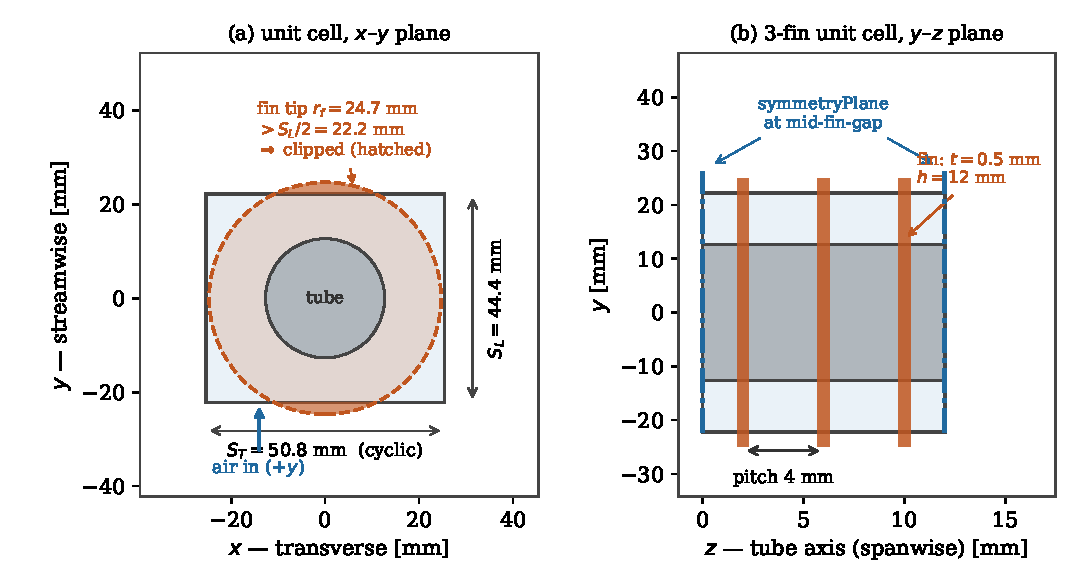
\includegraphics[width=\linewidth]{figs/fig_geometry.pdf}
\caption{The simulated unit cell. \textbf{(a)} Streamwise--transverse section: the meshed background box spans
$\pm S_T/2$ by $\pm S_L/2$, but the fin envelope of radius $r_f = 24.7$\,mm overruns it in $y$, so the hatched
crescents of fin metal are cut away by the inlet and outlet planes. \textbf{(b)} The three fins stacked along
the tube axis, closed by symmetry planes sitting at exact mid-fin-gap locations. \emph{The $z$ axis in (b) is
exaggerated} --- 12\,mm of $z$ against 49\,mm of $y$ is unreadable at true scale.}
\label{fig:geom}
\end{figure}


\section{Computational domain and mesh}

\subsection{Background block}

A single hex block, centred on the tube axis at $(x,y)=(0,0)$:

\begin{table}[h]\centering\small
\caption{\file{system/blockMeshDict} extents. Base grid $40\times34\times9$ cells, \file{simpleGrading (1 1 1)},
giving a base cell of $\approx d_o/20 \approx 1.27$\,mm.}\label{tab:block}
\begin{tabular}{@{}llll@{}}
\toprule
Direction & Extent (m) & Physical meaning & Length\\
\midrule
$x$ & $-0.0254 \ldots +0.0254$ & $\pm S_T/2$ (transverse) & 50.80\,mm\\
$y$ & $-0.022225 \ldots +0.022225$ & $\pm S_L/2$ (streamwise) & 44.45\,mm\\
$z$ & $0.0 \ldots 0.012$ & $3\times p_\mathrm{fin}$ (spanwise, tube axis) & 12.00\,mm\\
\bottomrule
\end{tabular}
\end{table}

\begin{table}[h]\centering\small
\caption{Boundary patches.}\label{tab:patches}
\begin{tabular}{@{}llll@{}}
\toprule
Patch & Type & Face & Role\\
\midrule
\file{inlet} & patch & $y=y_\mathrm{min}$ & air enters in $+y$\\
\file{outlet} & patch & $y=y_\mathrm{max}$ & air exits\\
\file{cyclicX\_neg} / \file{cyclicX\_pos} & cyclic pair & $x=x_\mathrm{min}$ / $x_\mathrm{max}$ & transverse periodicity of the bank\\
\file{symZ\_neg} / \file{symZ\_pos} & symmetryPlane & $z=z_\mathrm{min}$ / $z_\mathrm{max}$ & spanwise closure at mid-fin-gap\\
\file{tube} & wall (from snappy) & STL surface & the finned-tube surface\\
\bottomrule
\end{tabular}
\end{table}

\textbf{Why symmetryPlane and not cyclic in $z$.} The planes $z=0$ and $z=12$\,mm sit at exact symmetry planes
of the fin array (mid-gap between fins). Because the tube axis lies \emph{along} $z$, the wall crosses these
planes; symmetry is layer-meshable there where cyclic is not, and for this configuration the two are
physically identical. $z$ is a closure direction, not a streamwise-periodic bundle direction.

\subsection{snappyHexMesh}

Castellate, snap, and add layers, carving the STL out of the background box.

\begin{itemize}[leftmargin=1.4em,itemsep=1pt]
\item \textbf{Surface refinement} \file{level (2 3)}, giving 0.16--0.32\,mm on the general tube surface;
feature edges (\file{tube.eMesh}) at \file{level 3}.
\item \textbf{Gap refinement} \file{gapLevel (4 1 4)} drives the thin 0.5\,mm fins (tip and faces) to level~4
($\approx$0.08\,mm), so at least 4 cells span the fin thickness. Without this the fin tips sit on 0.32\,mm
cells and reach $y^+\approx7$ at the shoulders.
\item \file{nCellsBetweenLevels 2}, \file{resolveFeatureAngle 30}, \file{maxGlobalCells 4000000}.
\item \file{locationInMesh (0.023 0.020 0.0005)} --- a domain corner firmly in the air, outside the finned
envelope ($|(0.023, 0.020)| = 0.0305\,\mathrm{m} > r_f = 0.0247$\,m).
\item \textbf{Boundary layers on \file{tube}:} \file{nSurfaceLayers 8}, \file{expansionRatio 1.2},
\file{relativeSizes true}, \file{finalLayerThickness 0.3} (thinner first cell, $\approx$24\,$\mu$m, for $y^+$
margin), \file{minThickness 0.008}, \file{featureAngle 170} so layers wrap around the convex fin edges.
\end{itemize}

Feature extraction uses \file{extractFromSurface} with \file{includedAngle 150}; \file{nonManifoldEdges no},
\file{openEdges no} (the tube ends lie on symmetry planes, so no feature belongs there). Mesh quality limits
are OpenFOAM defaults tuned for wall-resolved layers: \file{maxNonOrtho 65} (relaxed 75),
\file{maxBoundarySkewness 20}, \file{maxInternalSkewness 4}, \file{maxConcave 80}, \file{minVol 1e-14}
(permitting thin layer cells), \file{minTetQuality 1e-15}, \file{minTwist 0.02}, \file{minDeterminant 0.001},
\file{minFaceWeight 0.02}, \file{minVolRatio 0.01}, \file{nSmoothScale 4}, \file{errorReduction 0.75}.

\subsection{The resulting mesh}

\begin{table}[h]\centering\small
\caption{Measured mesh metrics (\file{log.checkMesh}, \file{constant/polyMesh/boundary}).}\label{tab:mesh}
\begin{tabular}{@{}lr@{}}
\toprule
Metric & Value\\
\midrule
Total cells & \textbf{3\,288\,913} ($\approx$3.29\,M)\\
Hexahedra / prisms / polyhedra & 3\,092\,437 / 4\,872 / 191\,308\\
Max aspect ratio & 22.44 --- OK\\
Max non-orthogonality & 64.84 (average 7.08) --- OK\\
Max skewness & 3.05 --- OK\\
\file{checkMesh} verdict & \textbf{Mesh OK}\\
\file{tube} patch & 329\,016 faces, $9.0165\times10^{-3}$\,m$^2$ wetted\\
\file{inlet} / \file{outlet} & 9\,828 faces each\\
\bottomrule
\end{tabular}
\end{table}


\section{Boundary conditions and physics setup}

\subsection{Field boundary conditions}

\begin{table}[h]\centering\scriptsize
\caption{Field boundary conditions (\file{0.orig/}). Air enters in $+y$ at 740\,K and $\sim$2\,bar; the finned
tube is an isothermal 1033\,K no-slip wall.}\label{tab:bc}
\setlength{\tabcolsep}{4pt}
\resizebox{\linewidth}{!}{%
\begin{tabular}{@{}lllllll@{}}
\toprule
Field & internalField & \file{inlet} & \file{outlet} & \file{tube} & \file{cyclicX} & \file{symZ}\\
\midrule
$U$ [m/s] & (0 6.3623 0) & fixedValue & pressureInletOutletVelocity & noSlip & cyclic & symmetryPlane\\
$T$ [K] & 740 & fixedValue 740 & inletOutlet (740) & \textbf{fixedValue 1033} & cyclic & symmetryPlane\\
$p$ [Pa] & 2.0e5 & zeroGradient & fixedValue 2.0e5 & zeroGradient & cyclic & symmetryPlane\\
$k$ [m$^2$/s$^2$] & 0.1518 & fixedValue 0.1518 & inletOutlet & kqRWallFunction & cyclic & symmetryPlane\\
$\omega$ [1/s] & 280 & fixedValue 280 & inletOutlet & omegaWallFunction & cyclic & symmetryPlane\\
$\nu_t$ [m$^2$/s] & 0 & calculated & calculated & nutUSpaldingWallFunction & cyclic & symmetryPlane\\
$\alpha_t$ & 0 & calculated & calculated & alphatWallFunction ($Pr_t$ 0.85) & cyclic & symmetryPlane\\
\bottomrule
\end{tabular}}
\end{table}

Inlet turbulence is specified at intensity $I=5\%$ with length scale $L = 0.1\,d_o = 2.54$\,mm:
\begin{equation}
k = \tfrac32 (I\,U_\mathrm{in})^2 = 0.1518\ \mathrm{m^2/s^2},
\qquad
\omega = \frac{\sqrt{k}}{C_\mu^{1/4} L} = \frac{\sqrt{0.1518}}{0.09^{0.25}\times0.00254} \approx 280\ \mathrm{s^{-1}}.
\end{equation}

The wall treatment is low-Reynolds and wall-resolved. \file{nutUSpaldingWallFunction} and
\file{omegaWallFunction} are the $k$--$\omega$ SST \emph{blended} wall functions, valid continuously from the
viscous sublayer through the log layer --- so they remain correct even where the local $y^+$ exceeds the
$\leq2$ target (see \S\ref{sec:limits}). Turbulent Prandtl number $Pr_t = 0.85$.

\subsection{Thermophysical properties}

\begin{center}\small
\begin{minipage}{0.92\linewidth}\ttfamily\footnotesize
thermoType: hePsiThermo / pureMixture / sutherland transport / janaf thermo\\
\phantom{thermoType: }/ perfectGas equationOfState / sensibleEnthalpy\\
molWeight = 28.96 g/mol (air) $\rightarrow$ R = 287 J/kg$\cdot$K\\
Sutherland: mu = As$\cdot$T\^{}1.5/(T + Ts), As = 1.458e-6, Ts = 110.4 K\\
JANAF cp: Tlow 200 / Thigh 2500 / \textbf{Tcommon 1500 K}\\
\phantom{JANAF cp: }highCpCoeffs (3.09 0.00124 -4.2e-7 6.7e-11 -3.9e-15 -996 5.34)\\
\phantom{JANAF cp: }lowCpCoeffs (3.57 -7.2e-4 1.66e-6 -6.6e-10 5.1e-14 -1047 3.72)
\end{minipage}
\end{center}

\warnbox{A numerical trap worth knowing about.}{\file{Tcommon} was deliberately raised to \textbf{1500\,K},
above the entire operating and transient band of 740--1033\,K. The two JANAF coefficient sets are about 1\%
discontinuous in enthalpy at their join. With the default \file{Tcommon = 1000 K} sitting \emph{inside} the
operating range, the $T(h)$ Newton inversion oscillated across that jump and would not converge. Pushing
\file{Tcommon} above the band forces the whole domain onto one smooth coefficient set.}

Turbulence is RANS \file{kOmegaSST} with \file{turbulence on}. \file{constant/fvOptions} applies
\file{limitTemperature} over the whole domain with min 300\,K / max 1200\,K --- a \emph{transient-safety}
limiter that prevents an early SIMPLE iterate from driving a cell outside the JANAF range. At convergence the
field is physical (maximum wall-adjacent $T \leq 1033$\,K) and the limiter is dormant.


\section{Numerical method, execution, and convergence}

\subsection{Schemes and linear solvers}

Steady compressible pressure-based SIMPLE (\file{rhoSimpleFoam}).

\begin{itemize}[leftmargin=1.4em,itemsep=1pt]
\item \textbf{ddt:} \file{steadyState}. \textbf{grad:} \file{Gauss linear}, with \file{cellLimited Gauss
linear 1} on $U$, $e$, $h$, $k$, $\omega$.
\item \textbf{div:} \file{bounded Gauss linearUpwind grad(U)} for momentum and energy; \file{bounded Gauss
upwind} for $k$, $\omega$, and \file{div(phiv,p)}.
\item \textbf{laplacian:} \file{Gauss linear corrected}; \textbf{snGrad:} \file{corrected};
\textbf{wallDist:} \file{meshWave}.
\item \textbf{Linear solvers:} $p$ via GAMG/GaussSeidel (tol $10^{-8}$, relTol 0.05);
$(U|e|h|k|\omega)$ via PBiCGStab/DILU (tol $10^{-8}$, relTol 0.1).
\item \textbf{SIMPLE:} \file{consistent yes} (SIMPLEC), \file{nNonOrthogonalCorrectors 2}, residualControl
$10^{-4}$ on all of $p$, $U$, $e$, $h$, $k$, $\omega$.
\item \textbf{Relaxation:} fields $p$ 0.3, $\rho$ 0.05; equations $U$ 0.5, $e$ 0.5, $h$ 0.5, $(k|\omega)$ 0.5.
\end{itemize}

\subsection{Run configuration and in-run diagnostics}

\file{controlDict}: \file{endTime 2000}, \file{deltaT 1}, \file{writeInterval 100}, \file{purgeWrite 2},
\file{writeFormat ascii}, \file{writePrecision 8}, \file{runTimeModifiable true}. Function objects:

\begin{itemize}[leftmargin=1.4em,itemsep=1pt]
\item \file{yPlus1} --- $y^+$ on all walls at write time.
\item \file{wallHeatFlux1} --- wall heat flux and integral heat rate $Q$ over the \file{tube} patch. This is
the primary measurement from which $h$ is derived.
\item \file{fieldMinMax1} --- min/max of $U$, $p$, $T$ every 50 steps, as a physicality check.
\item \file{pIn} / \file{pOut} --- area-averaged static pressure on inlet and outlet every step, for the
streamwise $\Delta p$.
\end{itemize}

The mesh is decomposed into 10 subdomains by \file{scotch} and solved in parallel. All OpenFOAM commands run
inside the ESI image \file{opencfd/openfoam-default:2406} via Docker, with the \file{cfd/} tree mounted at
\file{/cfd}.

\warnbox{Docker quirk that costs an afternoon if you hit it cold.}{The OpenFOAM image's \file{ENTRYPOINT}
\file{cd}s to \file{\$HOME} before running the given command, so \file{docker run -w} (working directory) is
\emph{silently ignored}. The wrapper \file{run/of.sh} works around this by \file{cd}-ing to the case directory
\emph{inside} the shell command passed to the container, derived from the caller's path relative to the
\file{cfd/} root.}

The full pipeline (\file{run/Allrun}):
\begin{center}\ttfamily\footnotesize
blockMesh $\rightarrow$ surfaceFeatureExtract $\rightarrow$ snappyHexMesh -overwrite $\rightarrow$ checkMesh\\
$\rightarrow$ cp -r 0.orig 0 $\rightarrow$ decomposePar $\rightarrow$ mpirun -np 10 rhoSimpleFoam -parallel
$\rightarrow$ reconstructPar -latestTime
\end{center}

\subsection{Convergence}

SIMPLE converged in \textbf{464 iterations}, at which point the largest monitored initial residual was
$9.8\times10^{-5}$, just inside the $10^{-4}$ residualControl threshold that terminated the run
(Figure~\ref{fig:res}).

\begin{figure}[h]\centering
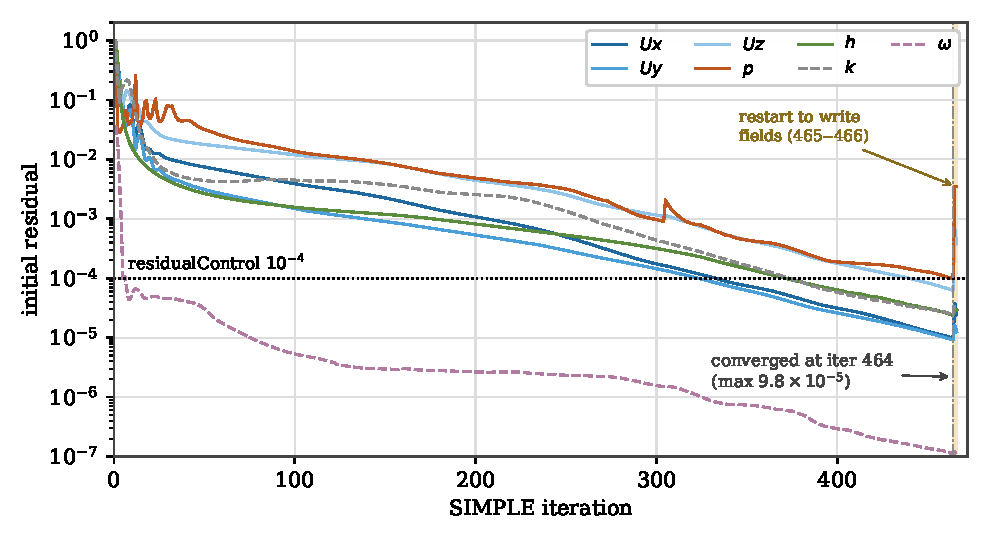
\includegraphics[width=0.92\linewidth]{figs/fig_residuals.pdf}
\caption{Convergence history, parsed directly from the solver logs. All seven solved fields fall monotonically
below the $10^{-4}$ residualControl gate by iteration 464. The step at iteration $\sim$300 is a clean restart
from a written checkpoint. The shaded band at 465--466 is a short restart used to re-write the fields and
function-object outputs from which the measurements were taken: the pressure residual shows the usual
restart transient there, but the measured quantity of interest is unaffected --- the integral wall heat rate
$Q$ differs between iterations 465 and 466 by 0.002\%.}
\label{fig:res}
\end{figure}

Measured $y^+$ on the \file{tube} patch at convergence: minimum $6.60\times10^{-4}$, \textbf{mean 0.244},
maximum 4.63. The mean satisfies the project's $y^+\leq2$ wall-resolution gate; the maximum exceeds it locally
at the fin leading-edge tips, discussed in \S\ref{sec:limits}.


\section{Post-processing and validation}

\subsection{Measured CFD quantities}

\begin{table}[h]\centering\small
\caption{Converged measurements (Time 466), frozen as documented constants in
\file{validation/single\_point\_check.py} so the Python reduction reproduces without re-running the CFD.}
\label{tab:measured}
\begin{tabular}{@{}lllr@{}}
\toprule
Quantity & Symbol & Value & Source\\
\midrule
Integral wall heat rate over \file{tube} & $Q$ & \textbf{256.30\,W} & \file{wallHeatFlux1}\\
Measured wetted area of \file{tube} & $A_\mathrm{wetted}$ & $9.0165\times10^{-3}$\,m$^2$ & 329\,016 faces (fin-clipped)\\
Streamwise pressure drop & $\Delta p$ & 148.4\,Pa & \file{pIn} / \file{pOut} probes\\
Wall / inlet temperature & $T_\mathrm{wall}$ / $T_\mathrm{in}$ & 1033 / 740\,K & boundary condition (input)\\
Inlet velocity / area & $U_\mathrm{in}$ / $A_\mathrm{inlet}$ & 6.3623\,m/s / $5.773\times10^{-4}$\,m$^2$ & BC / mesh\\
$y^+$ mean / max on \file{tube} & --- & 0.244 / 4.63 & \file{yPlus1}\\
Streamwise tube rows in domain & $N_\mathrm{rows}$ & 1 & single-tube unit cell\\
\bottomrule
\end{tabular}
\end{table}

\subsection{Reduction to Nusselt and friction numbers}

The property model is stated explicitly and reused everywhere for consistency: $\rho = p/(RT)$ with
$R=287$\,J/kg$\cdot$K; $\mu$ from Sutherland; $c_p = 1080$\,J/kg$\cdot$K (representative high-temperature air);
and $Pr = 0.69$ as an \emph{explicit choice}, so that $k_\mathrm{air} = \mu c_p / Pr$ rather than a separately
derived number. This keeps $Nu = h\,d_o/k_\mathrm{air}$ consistent with the same $Pr$ fed to the Briggs--Young
correlation. Properties are evaluated at the film temperature
$T_\mathrm{film} = (T_\mathrm{wall}+T_\mathrm{bulk,mean})/2$.

\begin{enumerate}[leftmargin=1.6em,itemsep=1pt]
\item $\rho_\mathrm{in} = p/(RT_\mathrm{in})$, \ $\mdot = \rho_\mathrm{in} U_\mathrm{in} A_\mathrm{inlet}$.
\item $T_\mathrm{out} = T_\mathrm{in} + Q/(\mdot c_p)$; \ $T_\mathrm{bulk,mean} = (T_\mathrm{in}+T_\mathrm{out})/2$;
\ $T_\mathrm{film} = (T_\mathrm{wall}+T_\mathrm{bulk,mean})/2$.
\item Area-averaged wall flux $q'' = Q/A_\mathrm{wetted}$.
\item Two candidate $\Delta T$ conventions for $h$ --- and the choice is material:
\[
h_\mathrm{inlet} = \frac{q''}{T_\mathrm{wall}-T_\mathrm{in}} \ \Rightarrow\ Nu = 40.3,
\qquad
h_\mathrm{LMTD} = \frac{q''}{\mathrm{LMTD}} \ \Rightarrow\ \mathbf{Nu = 45.9},
\]
\[
\text{with}\quad
\mathrm{LMTD} = \frac{\Delta T_\mathrm{in}-\Delta T_\mathrm{out}}
{\ln(\Delta T_\mathrm{in}/\Delta T_\mathrm{out})},\quad
\Delta T_\mathrm{in}=T_\mathrm{wall}-T_\mathrm{in},\ \
\Delta T_\mathrm{out}=T_\mathrm{wall}-T_\mathrm{out}.
\]
\item Reynolds number at the minimum-flow section: $G_\mathrm{max} = \mdot/A_\mathrm{min}$,
$Re = G_\mathrm{max} d_o/\mu(T_\mathrm{film}) = 8368$.
\item Friction factor as an Euler number per row:
$f_\mathrm{CFD} = \Delta p / (\tfrac12 \rho_\mathrm{in} U_\mathrm{max}^2 N_\mathrm{rows}) = 1.688$.
\end{enumerate}

\subsection{The published correlations}

\begin{align}
\text{Briggs \& Young (1963):}\quad
Nu &= 0.134\,Re^{0.681}Pr^{1/3}
      \left(\frac{s}{h_\mathrm{fin}}\right)^{0.2}
      \left(\frac{s}{t_\mathrm{fin}}\right)^{0.1134},
      \quad s = p_\mathrm{fin}-t_\mathrm{fin}\\[2pt]
\text{Robinson \& Briggs (1966):}\quad
f &= 9.465\,Re^{-0.316}\left(\frac{S_T}{d_o}\right)^{-0.927}
\end{align}
Evaluated at $Re = 8368$ for this geometry: $Nu_\mathrm{BY} = 54.1$ and $f_\mathrm{RB} = 0.287$.

\subsection{The validation result}

\begin{table}[h]\centering\small
\caption{CFD versus published correlations at $Re = 8368$.}\label{tab:valid}
\begin{tabular}{@{}lrrrl@{}}
\toprule
Quantity & CFD & Correlation & Deviation & Verdict\\
\midrule
\textbf{$Nu$ (LMTD $\Delta T$)} & \textbf{45.9} & 54.1 & \textbf{$-15.2\%$} & within $\pm20\%$ $\rightarrow$ \textbf{heat transfer VALIDATED}\\
$Nu$ (inlet $\Delta T$) & 40.3 & 54.1 & $-25.5\%$ & outside $\pm20\%$ (wrong $\Delta T$ convention)\\
\textbf{$f$ (friction)} & \textbf{1.688} & 0.287 & \textbf{$+489\%$} & outside $\pm20\%$ $\rightarrow$ \textbf{does NOT validate}\\
\bottomrule
\end{tabular}
\end{table}

\begin{figure}[h]\centering
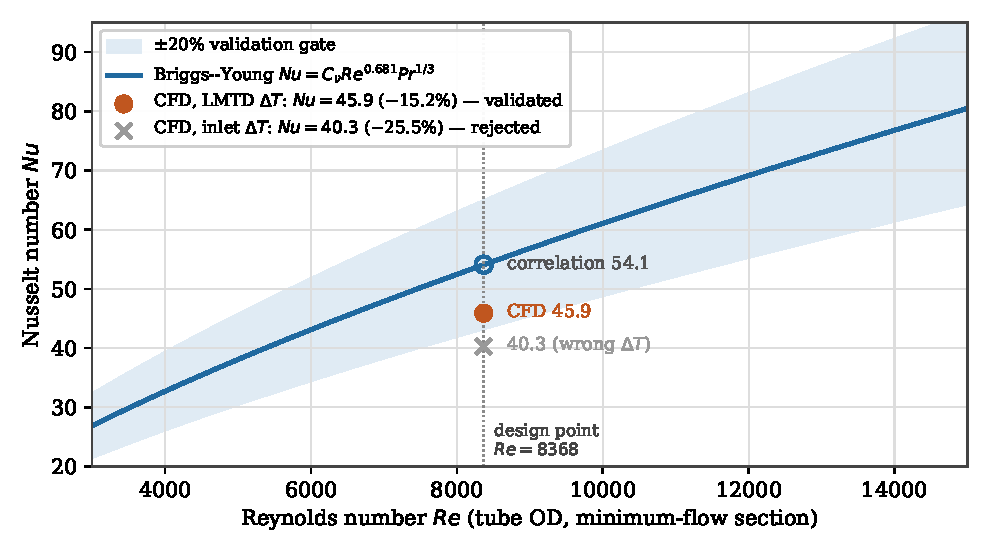
\includegraphics[width=0.86\linewidth]{figs/fig_nu_validation.pdf}
\caption{The validation. The CFD point evaluated with the log-mean temperature difference falls inside the
$\pm20\%$ engineering gate around the Briggs--Young correlation; the same CFD run reduced with the naive
wall-minus-inlet $\Delta T$ falls outside it. One simulation, two answers --- which is why the $\Delta T$
convention had to be argued rather than assumed.}
\label{fig:nu}
\end{figure}

\textbf{Why LMTD and not inlet-$\Delta T$.} The air bulk-warms appreciably across the cell, so the log-mean
driving temperature difference is the physically correct mean for an integrated heat-exchanger balance --- and
it is the basis on which the Briggs--Young correlation itself was constructed. Using the simpler
wall-minus-inlet $\Delta T$ overstates the driving temperature difference, understates $h$, and drops $Nu$ to
40.3. Comparing an inlet-$\Delta T$ Nusselt number against an LMTD-based correlation would not be a like-for-like
comparison. The convention is material and was chosen on physical grounds, not to pass the gate.

\textbf{Why friction misses, and why it is not fatal.} The discrepancy is not a Reynolds-dependence problem
that a sweep would resolve --- it is a \emph{measurement-domain mismatch}. The CFD $\Delta p$ spans the entire
unit cell: inlet plenum, tube, and outlet wake, roughly 1.7 velocity heads. Robinson--Briggs describes only
the incremental per-row loss inside a fully developed multi-row bank. The two quantities are not measuring the
same thing. Fin clipping (\S\ref{sec:limits}) compounds this by adding spurious form drag on the CFD side.
Heat transfer validates cleanly because it is dominated by the well-resolved bulk boundary layer (mean
$y^+ = 0.244$) rather than by entrance and exit geometry. Friction is therefore reported as informational and
is \textbf{not} wired into the v2 power balance.


\section{Constructing the $UA(\dot m)$ law}
\label{sec:ualaw}

Heat transfer having validated, the now-CFD-validated Briggs--Young $Nu(Re)$ law is adopted as the air-side
model and converted into an overall heater conductance. Reynolds number tracks mass flow linearly
($Re = Re_\mathrm{des}\,\mdot/\mdot_\mathrm{des}$), and the law is \emph{anchored} so that v2 reproduces v1.5
exactly at the design point:
\begin{equation}
UA(\mdot) \;=\; UA_\mathrm{des}\;
\underbrace{\frac{Nu(\mdot)}{Nu_\mathrm{des}}}_{\text{raw } \propto\, \mdot^{0.681}}\;
\underbrace{\frac{\eta_o\big(h(\mdot)\big)}{\eta_o(h_\mathrm{des})}}_{\text{fin-efficiency modulation}},
\qquad
\eta_o = 1 - \frac{A_\mathrm{fin}}{A_\mathrm{tot}}\Big(1-\eta_\mathrm{fin}(h)\Big).
\label{eq:ualaw}
\end{equation}
with $UA_\mathrm{des} = 152.35$\,kW/K at $\mdot_\mathrm{des} = 54.37$\,kg/s, both taken live from
\file{cycle\_model.\allowbreak hx\_entu\_v1\_5.\allowbreak size\_design}
so the anchor cannot drift out of sync.

\keybox{The most interesting physics in this report.}{The raw heat-transfer scaling is \emph{steeper} than
v1.5's assumption ($h\propto Re^{0.681}$ against the assumed $0.6$), so the expectation going in was that the
CFD would push the exponent up to 0.66--0.68. It did the opposite. Because $UA = h A \eta_o$ and the reference
fin is thermally \textbf{inefficient} ($\eta_\mathrm{fin}\approx0.53$ at design --- realistic for a
low-conductivity $k\approx25$\,W/m$\cdot$K high-temperature alloy fin), driving the fin harder makes it worse:
a larger root-to-tip temperature drop lowers its efficiency. So $\eta_o$ \emph{falls} as $\mdot$ rises, from
0.62 to 0.54 across the swept range, contributing $\mathrm{d}\ln\eta_o/\mathrm{d}\ln\mdot \approx -0.23$. That
modulation dominates: $0.681 - 0.23 \approx \mathbf{0.454}$, \emph{shallower} than the assumed 0.6.}

\begin{figure}[h]\centering
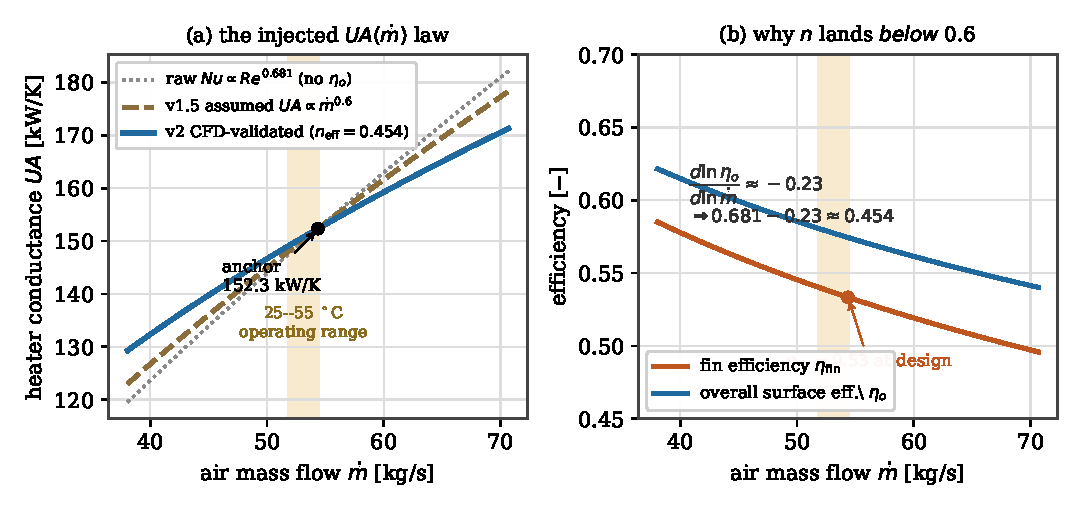
\includegraphics[width=\linewidth]{figs/fig_ua_law.pdf}
\caption{\textbf{(a)} The injected law against v1.5's assumption, all anchored at the same design point. The
shaded strip is the mass-flow range the cycle actually visits across 25--55\,\co{} --- note how narrow it is
relative to the range over which the laws differ. \textbf{(b)} Why the effective exponent lands below 0.6:
the annular fin's efficiency is low and falls with increasing $h$, dragging the overall surface efficiency
$\eta_o$ down as mass flow rises and cancelling most of the steeper raw Nusselt scaling.}
\label{fig:ua}
\end{figure}

A least-squares log-log fit of Eq.~\ref{eq:ualaw} over $\mdot = 0.7\ldots1.3\,\mdot_\mathrm{des}$ gives the
effective exponent $n_\mathrm{air,eff} = \mathbf{0.4539}$.

\subsection{The interface artifact}

The law is emitted as \file{phase1\_derating/cfd/results/cfd\_correlation.json}, the single file that carries
the CFD result into the cycle model.

\begin{table}[h]\centering\small
\caption{Contents of \file{cfd\_correlation.json}.}\label{tab:json}
\resizebox{\linewidth}{!}{%
\begin{tabular}{@{}llp{7.6cm}@{}}
\toprule
Key & Value & Meaning\\
\midrule
\file{C\_nu} & 0.13059 & geometry coefficient in $Nu = C_\nu Re^m Pr^{1/3}$\\
\file{m} & 0.681 & Briggs--Young Reynolds exponent\\
\file{C\_f}, \file{p} & 4.9781, $-0.316$ & Robinson--Briggs friction --- \emph{informational only}\\
\file{Re\_des} & 8368 & design / validation Reynolds number\\
\file{Pr} & 0.69 & Prandtl number (modelling choice)\\
\file{k\_air\_des} & 0.061133\,W/m$\cdot$K & air conductivity at design film temperature\\
\file{UA\_design\_kW\_per\_K} & 152.349 & v1.5 anchor magnitude\\
\file{mdot\_des\_kg\_s} & 54.370 & v1.5 anchor mass flow\\
\file{n\_air\_effective} & 0.4539 & effective $UA\propto\mdot^{\,n}$ (against v1.5's 0.6)\\
\file{n\_tubes} & 1281.4 & \textbf{diagnostic only} --- tube count at $L=2.0$\,m reproducing $UA_\mathrm{des}$;
  not a plant specification\\
\file{validation} & $\{45.9, 54.1, -15.2\%; 1.688, 0.287, +489\%\}$ & frozen single-point outcome\\
\bottomrule
\end{tabular}}
\end{table}


\section{Results}

\subsection{The v2 derating curve}

\file{cfd\_to\_v2.py} injects the law of Eq.~\ref{eq:ualaw} into the v1.5 cycle model in place of its
\file{ua\_law} hook and regenerates the curve over 25--55\,\co. The mechanism is a single substitution --- the
cycle model, reactor, and control logic are otherwise untouched, which is what makes v2 a clean test of the
heater law alone rather than of a rewritten model.

\begin{table}[h]\centering\small
\caption{The v2 curve at key ambient temperatures. Regime B is the fixed-design regime; regime A is the hotter
regime in which the required heat-pipe source temperature hits its ceiling and heat must be shed.}
\label{tab:v2}
\begin{tabular}{@{}rrrcrrr@{}}
\toprule
Ambient & $\mdot$ (kg/s) & TIT (\co) & Regime & net MW$_\mathrm{e}$ & \% of 25\,\co & plant $\eta$\\
\midrule
25\,\co & 54.370 & 742 & B & 5.000 & 100.0\% & 0.333\\
35\,\co & 53.480 & 762 & B & 4.926 & 98.5\% & 0.328\\
45\,\co & 52.633 & 782 & A & 4.852 & 97.1\% & 0.323\\
55\,\co & 51.825 & 783 & A & 4.566 & 91.3\% & 0.304\\
\bottomrule
\end{tabular}
\end{table}

Mean electric derating over 25--45\,\co{} is 0.15\%/\co, and the penalty at 55\,\co{} is $\mathbf{-8.7\%}$.

\subsection{v2 against v1.5: the curve does not move}

\begin{figure}[h]\centering
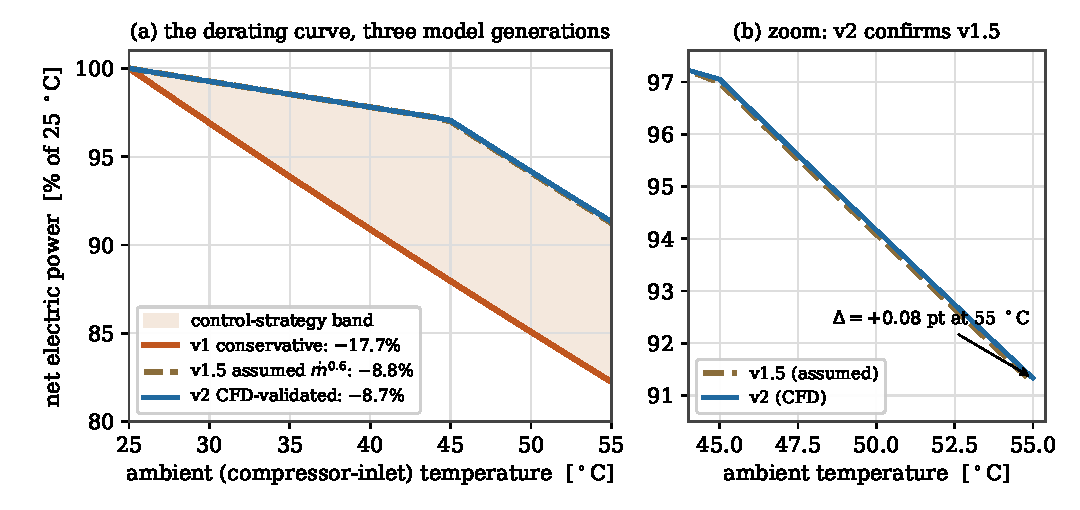
\includegraphics[width=\linewidth]{figs/fig_derating.pdf}
\caption{\textbf{(a)} The three model generations. v1 and v2 bracket the answer as a control-strategy band:
the difference between them is not modelling uncertainty but a genuine choice about whether the plant holds
firing temperature fixed or lets it float as ambient rises. \textbf{(b)} The point of this campaign, zoomed:
replacing the assumed air-side law with the CFD-validated one leaves the curve essentially where it was.}
\label{fig:derate}
\end{figure}

\begin{table}[h]\centering\small
\caption{The headline comparison at 55\,\co.}\label{tab:vs}
\begin{tabular}{@{}lrr@{}}
\toprule
 & penalty @ 55\,\co & net MW$_\mathrm{e}$ @ 55\,\co\\
\midrule
v1.5 (assumed $UA\propto\mdot^{0.6}$) & $-8.75\%$ & 4.57\\
\textbf{v2 (CFD-validated, $n\approx0.454$)} & $\mathbf{-8.67\%}$ & 4.57\\
$\Delta$ (v2 $-$ v1.5) & \textbf{$+0.08$ pt} & $\approx0$\\
\bottomrule
\end{tabular}
\end{table}

\subsection{Why the curve does not move --- and why that is the result}
\label{sec:robust}

A 24\% change in the air-side exponent ($0.6 \rightarrow 0.454$) shifted the 55\,\co{} penalty by less than
one tenth of a percentage point. That demands an explanation, not a shrug, and the explanation is the
genuinely useful output of this campaign.

The reason is visible in Table~\ref{tab:v2}: air mass flow falls only from 54.37 to 51.83\,kg/s across the
entire 25$\rightarrow$55\,\co{} range --- about 4.7\%. The exponent $n$ acts on that ratio, so its influence
enters as $1.047^{\,n}$. Between $n = 0.454$ and $n = 0.6$ that is the difference between 1.021 and 1.028: a
0.7\% change in heater conductance, which the $\varepsilon$--NTU balance then dilutes further before it
reaches net power.

To make the claim quantitative rather than anecdotal, the cycle model was re-run with $UA\propto\mdot^{\,n}$
swept across the entire physically plausible range and beyond, $n \in [0, 1.2]$ --- from a heater whose
conductance ignores mass flow entirely to one that scales super-linearly with it (Figure~\ref{fig:sens}).

\begin{figure}[h]\centering
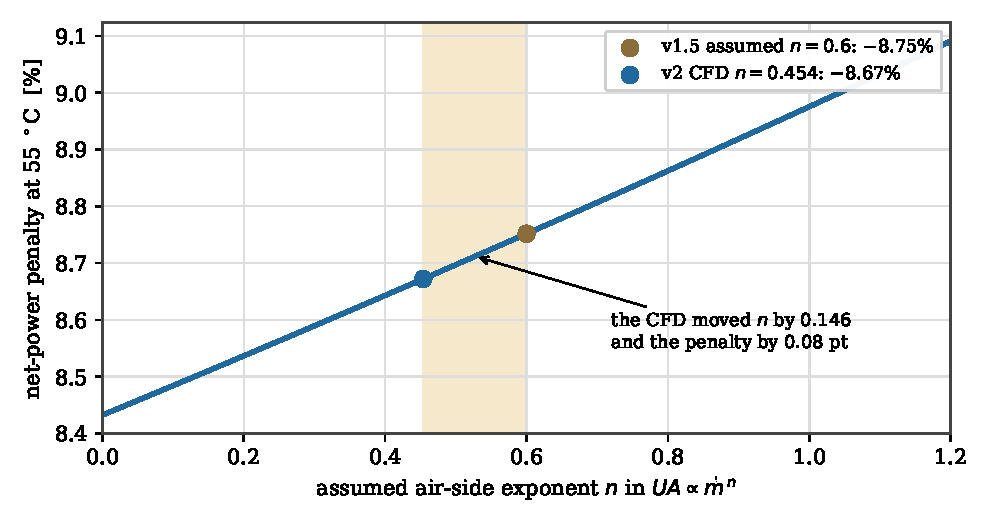
\includegraphics[width=0.86\linewidth]{figs/fig_sensitivity.pdf}
\caption{Sensitivity of the 55\,\co{} penalty to the assumed air-side exponent, computed by re-running the
cycle model 25 times. Across the full range $n\in[0,1.2]$ the penalty spans only 8.43--9.09\%, a total spread
of 0.66 percentage points. The distance the CFD actually moved the exponent is the shaded strip.}
\label{fig:sens}
\end{figure}

\keybox{The finding.}{Over the entire range $n \in [0,1.2]$, the 55\,\co{} penalty varies by just
\textbf{0.66 percentage points} (8.43\% to 9.09\%). The air-side heat-transfer law is a second-order term in
the desert derating problem. The penalty is set by compressor-inlet thermodynamics --- which v1 and v1.5
already captured --- and is \emph{robust} to the heater model.}

This reframes what the CFD delivered. It is not a corrected number; it is a \textbf{demonstrated
insensitivity}. Before this campaign, v1.5's $-8.8\%$ rested on an unverified textbook exponent, and a
reviewer would have been right to ask what happens if that exponent is wrong. The answer is now on the record,
computed from physics: almost nothing happens, and here is the range over which almost nothing happens. An
independent physics simulation confirming an assumption is a weaker headline than overturning one, but it is
the outcome that makes the Phase-1 curve defensible as a Phase-2 input.


\section{Honest limitations}
\label{sec:limits}

These are stated in full because a reader deciding how far to trust the result needs them, and because the
project's standard is that limitations are documented rather than discovered later by someone else.

\begin{enumerate}[leftmargin=1.6em,itemsep=3pt]
\item \textbf{Fin clipping.} $r_f = 24.7$\,mm exceeds $S_L/2 = 22.2$\,mm, so the 12\,mm fins overrun the
single-tube streamwise box and are clipped at the inlet and outlet planes --- about 42\% of the inlet plane is
fin metal at fin $z$-levels. This is inherent to the reference geometry (fin height $\approx$ tube radius)
combined with a single-tube box: one unit cell cannot represent the interleaving of staggered neighbouring
tubes' fins. It biases the \emph{friction} measurement by adding spurious clipped-fin form drag. Heat transfer
still validates at $-15.2\%$.

\item \textbf{Friction is not validated and is not used.} The Robinson--Briggs $\Delta p$ and
parasitic-power estimate is carried in \file{cfd\_correlation.json} for reference only and is excluded from
the v2 power balance. Fan parasitic power in v2 still comes from the cycle model's own treatment.

\item \textbf{Mesh independence was not formally studied.} A single validated point stands in for a
grid-convergence study, supported by \emph{adequacy evidence} --- the $-15.2\%$ Nusselt agreement, mean
$y^+ = 0.244$, and a clean \file{checkMesh} --- rather than by proof. A formal three-level grid-convergence
study is future work. This is the limitation most likely to be challenged in peer review.

\item \textbf{$\omega$ bounding at fin tips.} A localized near-singular-corner artifact in the $k$--$\omega$
solve at the fin leading edges. It does not perturb the converged $U$, $p$, or $T$ fields, and the integrated
$h$ and $f$ are bulk-dominated, so it does not affect the reported result.

\item \textbf{$y^+$ gate exceeded locally.} The project's mesh-quality gate is $y^+\leq2$ on tube and fin
walls. The mean (0.244) satisfies the wall-resolved intent of that gate, but the maximum (4.63) exceeds it at
the fin leading-edge tips --- the same near-singular corners behind limitation 4. The $k$--$\omega$ SST blended
wall functions remain valid at these $y^+$ values and the integrated $h$ is bulk-dominated, so the
heat-transfer validation stands.

\item \textbf{Option 1, not a full sweep.} This is a single-point validation plus a correlation-driven curve,
not a six-point CFD Reynolds sweep. The choice and its justification are recorded as decision D12.

\item \textbf{The heat-exchanger geometry is representative, not the real one.} eVinci's finned-tube
geometry is not public. The reference bank in Table~\ref{tab:geom} is a plausible standard specification, so
the CFD validates \emph{a} realistic air-side heater, not \emph{the} eVinci heater. Given the demonstrated
insensitivity of \S\ref{sec:robust}, this matters less for the derating result than it would otherwise.
\end{enumerate}


\section{How to reproduce}

\begin{center}\begin{minipage}{0.95\linewidth}\ttfamily\footnotesize
\# --- CFD (needs Docker + the ESI OpenFOAM v2406 image) ---\\
cd phase1\_derating/cfd\\
python3 -c "from geometry.finned\_tube import REFERENCE; \textbackslash\\
\phantom{python3 -c "}from geometry.make\_stl import write\_unitcell\_stl; \textbackslash\\
\phantom{python3 -c "}print(write\_unitcell\_stl(REFERENCE, 'heater\_unitcell/constant/triSurface/tube.stl'))"\\
run/Allrun \ \ \ \ \# mesh $\rightarrow$ checkMesh $\rightarrow$ parallel solve $\rightarrow$ reconstruct ($\sim$25 min, 10 cores)\\[4pt]
\# --- Post-processing / validation / injection (pure Python, no Docker) ---\\
python3 -m validation.single\_point\_check \ \ \# CFD vs correlations at Re=8368\\
python3 -m postprocessing.fit \ \ \ \ \ \ \ \ \ \ \ \# writes results/cfd\_correlation.json\\
python3 cfd\_to\_v2.py \ \ \ \ \ \ \ \ \ \ \ \ \ \ \ \ \ \# injects UA law $\rightarrow$ derating\_curve\_v2.csv\\
python3 -m pytest -q \ \ \ \ \ \ \ \ \ \ \ \ \ \ \ \ \ \# 21-test suite\\[4pt]
\# --- This report ---\\
python3 CFD\_Report/make\_figs.py \ \ \ \ \ \ \ \ \ \# regenerates all six figures from project data\\
cd CFD\_Report \&\& latexmk -pdf report.tex
\end{minipage}\end{center}

\textbf{What is version-controlled versus regenerated.} The OpenFOAM case \emph{source} is committed:
\file{system/} dictionaries, \file{constant/} property and turbulence files, \file{0.orig/} fields, and
\file{constant/triSurface/tube.stl}. Run artifacts --- \file{0/}, \file{processorN/},
\file{constant/polyMesh/}, \file{postProcessing/}, and logs --- are gitignored and regenerated by
\file{run/Allrun}. The frozen measured CFD scalars live as documented constants in
\file{validation/single\_point\_check.py} and \file{postprocessing/fit.py}, so the entire Python
validation and injection chain reproduces without access to a CFD-capable machine.

\warnbox{One maintenance hazard.}{The measured scalars in \file{validation/single\_point\_check.py} are
hardcoded from the converged run at Time 466. If the case is ever re-run with modified settings, those
constants will silently go stale --- nothing recomputes them automatically. Re-run
\file{python3 -m postprocessing.extract} against the new \file{postProcessing/} tree and update them
deliberately.}


\section{Future work}
\label{sec:future}

In priority order:

\begin{enumerate}[leftmargin=1.6em,itemsep=3pt]
\item \textbf{Intake/exhaust recirculation study --- the highest-value next step.} In a real desert skid, hot
turbine exhaust can be drawn back into the compressor intake, raising the effective inlet temperature
\emph{above} ambient and making the derating worse than any of the curves in this report. No correlation
covers this: it depends on skid layout, stack height, and local wind. It genuinely requires CFD, and the
validated air-side setup produced here is the foundation for it. It also feeds Phase~2 directly, since the
penalty becomes layout-dependent. It needs an assumed skid external geometry to proceed.
\item \textbf{Full multi-condition Reynolds sweep,} deriving $Nu(Re)$ entirely from simulation rather than
validating a published correlation.
\item \textbf{Fin-geometry sensitivity.} The reference fins are thermally inefficient
($\eta_\mathrm{fin}\approx0.53$); a better fin would change both the scaling and the heater size. Given
\S\ref{sec:robust}, this matters more for heat-exchanger design than for the derating curve.
\item \textbf{Formal three-level mesh-independence study,} for publication-grade rigour on the validated point.
\item \textbf{Friction-domain fix:} dedicated $\Delta p$ planes bracketing the bundle, or a multi-row domain,
so that friction can be validated and the parasitic-power estimate wired into the power balance.
\end{enumerate}


\appendix
\section{File map}

\begin{table}[h]\centering\small
\caption{Where everything lives, relative to the repository root.}\label{tab:files}
\setlength{\tabcolsep}{4pt}
\begin{tabular}{@{}lp{8.1cm}@{}}
\toprule
Path & Contents\\
\midrule
\file{phase1\_derating/cfd/README.md} & reproduction detail and directory layout\\
\file{\ldots/geometry/finned\_tube.py} & \file{FinnedTube}, \file{REFERENCE}, derived quantities, fin efficiency\\
\file{\ldots/geometry/make\_stl.py} & parametric STL generator for the 3-fin unit cell\\
\file{\ldots/correlations/finned\_tube\_corr.py} & Briggs--Young ($Nu$) and Robinson--Briggs ($f$)\\
\file{\ldots/heater\_unitcell/} & the OpenFOAM case: \file{system/}, \file{constant/}, \file{0.orig/}\\
\file{\ldots/run/of.sh}, \file{run/Allrun} & Docker wrapper and the full mesh-to-solve pipeline\\
\file{\ldots/postprocessing/extract.py} & parses \file{postProcessing/} into $h$, $\Delta p$, $f$\\
\file{\ldots/postprocessing/fit.py} & builds the $UA(\mdot)$ law, writes \file{cfd\_correlation.json}\\
\file{\ldots/validation/single\_point\_check.py} & CFD versus correlations at $Re = 8368$\\
\file{\ldots/cfd\_to\_v2.py} & injects the law into the cycle model\\
\file{\ldots/tests/} & 21-test pytest suite over geometry, correlations, extract, fit\\
\file{phase1\_derating/cycle\_model/hx\_entu\_v1\_5.py} & the v1.5 cycle model with the \file{ua\_law} hook\\
\file{phase1\_derating/results/derating\_curve\_v2.csv} & the v2 curve\\
\file{DECISIONS\_LOG.md} (entry D12) & the decision record and full rationale for Option 1\\
\file{CFD\_Report/make\_figs.py} & regenerates every figure in this report\\
\bottomrule
\end{tabular}
\end{table}

\section{Key numbers at a glance}

\begin{table}[h]\centering\small
\caption{Quick reference.}\label{tab:quick}
\begin{tabular}{@{}llr@{}}
\toprule
Category & Quantity & Value\\
\midrule
Operating point & Reynolds number & 8368\\
 & inlet air / wall temperature & 740 / 1033\,K\\
 & pressure & 2.0\,bar\\
Mesh & cells & 3\,288\,913\\
 & $y^+$ mean / max & 0.244 / 4.63\\
 & max non-orthogonality / skewness & 64.84 / 3.05\\
Convergence & iterations & 464\\
 & largest residual at stop & $9.8\times10^{-5}$\\
Measurement & integral wall heat rate $Q$ & 256.30\,W\\
 & pressure drop $\Delta p$ & 148.4\,Pa\\
Validation & $Nu$ CFD / correlation & 45.9 / 54.1 ($-15.2\%$) \textbf{pass}\\
 & $f$ CFD / correlation & 1.688 / 0.287 ($+489\%$) \textbf{fail}\\
$UA$ law & design anchor & 152.35\,kW/K @ 54.37\,kg/s\\
 & effective exponent (v2) & 0.454\\
 & assumed exponent (v1.5) & 0.600\\
 & fin efficiency at design & 0.533\\
Result & penalty @ 55\,\co, v1.5 / v2 & $-8.75\%$ / $-8.67\%$\\
 & sensitivity across $n\in[0,1.2]$ & 0.66\,pt total spread\\
\bottomrule
\end{tabular}
\end{table}

\section{References}

\begin{enumerate}[leftmargin=1.6em,itemsep=2pt]
\item Briggs, D.E. \& Young, E.H. (1963). \emph{Convection heat transfer and pressure drop of air flowing
across triangular pitch banks of finned tubes}. Chemical Engineering Progress Symposium Series.
\item Robinson, K.K. \& Briggs, D.E. (1966). \emph{Pressure drop of air flowing across triangular pitch banks
of finned tubes}. Chemical Engineering Progress Symposium Series.
\item IAEA Advanced Reactors Information System (ARIS), 2024 datasheet: Westinghouse eVinci microreactor.
\item OpenFOAM (ESI) v2406; container image \file{opencfd/openfoam-default:2406}. Python post-processing uses
numpy, pandas, matplotlib, and numpy-stl.
\end{enumerate}

\end{document}
